\documentclass{beamer}
%\documentclass[notes=only]{beamer}   % only notes
\usetheme[progressbar=foot]{metropolis}

% IMPORTS
\usepackage[ngerman]{babel}
\usepackage[utf8x]{inputenc}
\usepackage{parskip} 	% Absätze ohne Einrückungen
\usepackage{amsmath}
\usepackage{amssymb}
\usepackage{graphicx}	% Einbinden von Grafiken
\usepackage{float}		% figure: [H]
\usepackage{wrapfig}	% figure: [l]
\usepackage{subfigure}
\usepackage{caption}
\usepackage{url}
\usepackage{hyperref}

% Custom colors
\usepackage{xcolor}
\definecolor{deepblue}{RGB}{46,206,227}
\definecolor{deepred}{RGB}{245,20,66}
\definecolor{deepgreen}{RGB}{98,213,51}
\definecolor{deepgrey}{RGB}{183,183,183}
\definecolor{deepyellow}{RGB}{222,203,80}
\definecolor{commentgreen}{RGB}{78,139,70}

\usepackage{listings}

\lstset{ 
language=Python,
basicstyle=\ttfamily,
otherkeywords={self},                   % Add keywords here
keywordstyle=\ttfamily\color{deepblue},
emph={MyClass,__init__},                % Custom highlighting
emphstyle=\ttfamily\color{deepred},     % Custom highlighting style
stringstyle=\color{deepyellow},
commentstyle=\color{commentgreen},      % comment style
frame=tb,                               % Any extra options here
tabsize=2,
showstringspaces=false 
}

\title{Grundkurs: Programmieren}
\subtitle{Einführung in grundlegende Programmierkonzepte mit Python}
\date{\today}
\author{Christoph Sonntag}
\institute{Universität Passau}
\subject{Computer Science}

\begin{document}
\maketitle

\note[itemize]{
    \item kleine Vorstellung, wer ich bin, was ich mache (Name, Studium, Selbstständigkeit)
    \item Heute nur bis 18:00 Uhr, morgen um 10:00 Uhr, wann Mittagspause? Wie lange?
}

\section{Einführung in die Programmierung}

\begin{frame}{Erwartungen und Vorkenntnisse}
    \begin{itemize}
        \item Erwartungen an den Kurs?
        \item Bereits Programmierkenntnisse aus Schule/Universität?
        \item Kursziele 
            \begin{itemize}
                \item grundlegendes Verständnis
                \item ``mit Informatikern reden können"
                \item Angst nehmen
            \end{itemize}
    \end{itemize}
\end{frame}

\begin{frame}{Die Programmiersprache Python}
\begin{columns}
    \column{0.5\textwidth}
    \begin{itemize}
        \item Cool
    \end{itemize}
    \column{0.5\textwidth}
    \centering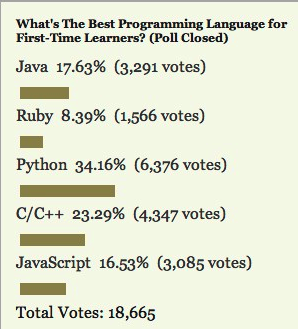
\includegraphics[scale=0.5]{images/best_lang} 
\end{columns}
\end{frame}



\end{document}
